\section{Results and Discussion}

This section presents the comprehensive results of our evaluation of Large Language Models (LLMs) for automated refactoring classification. We analyzed 2,728 commits from open-source Java projects, comparing the performance of three LLMs (Gemma-2:2b, Mistral, and DeepSeek-R1:8b) against the established Purity tool. Our analysis reveals both the potential and limitations of LLM-based approaches, providing insights into their applicability for software engineering tasks.

\subsection{Classification Distribution Analysis}

The distribution of classifications across different models reveals significant variations in how each approach categorizes refactoring commits. Figure~\ref{fig:classification-distribution} shows the proportion of PURE versus FLOSS classifications for each model, highlighting a clear trend toward more conservative (FLOSS) labeling by the LLMs.

\begin{figure}[H]
\centering
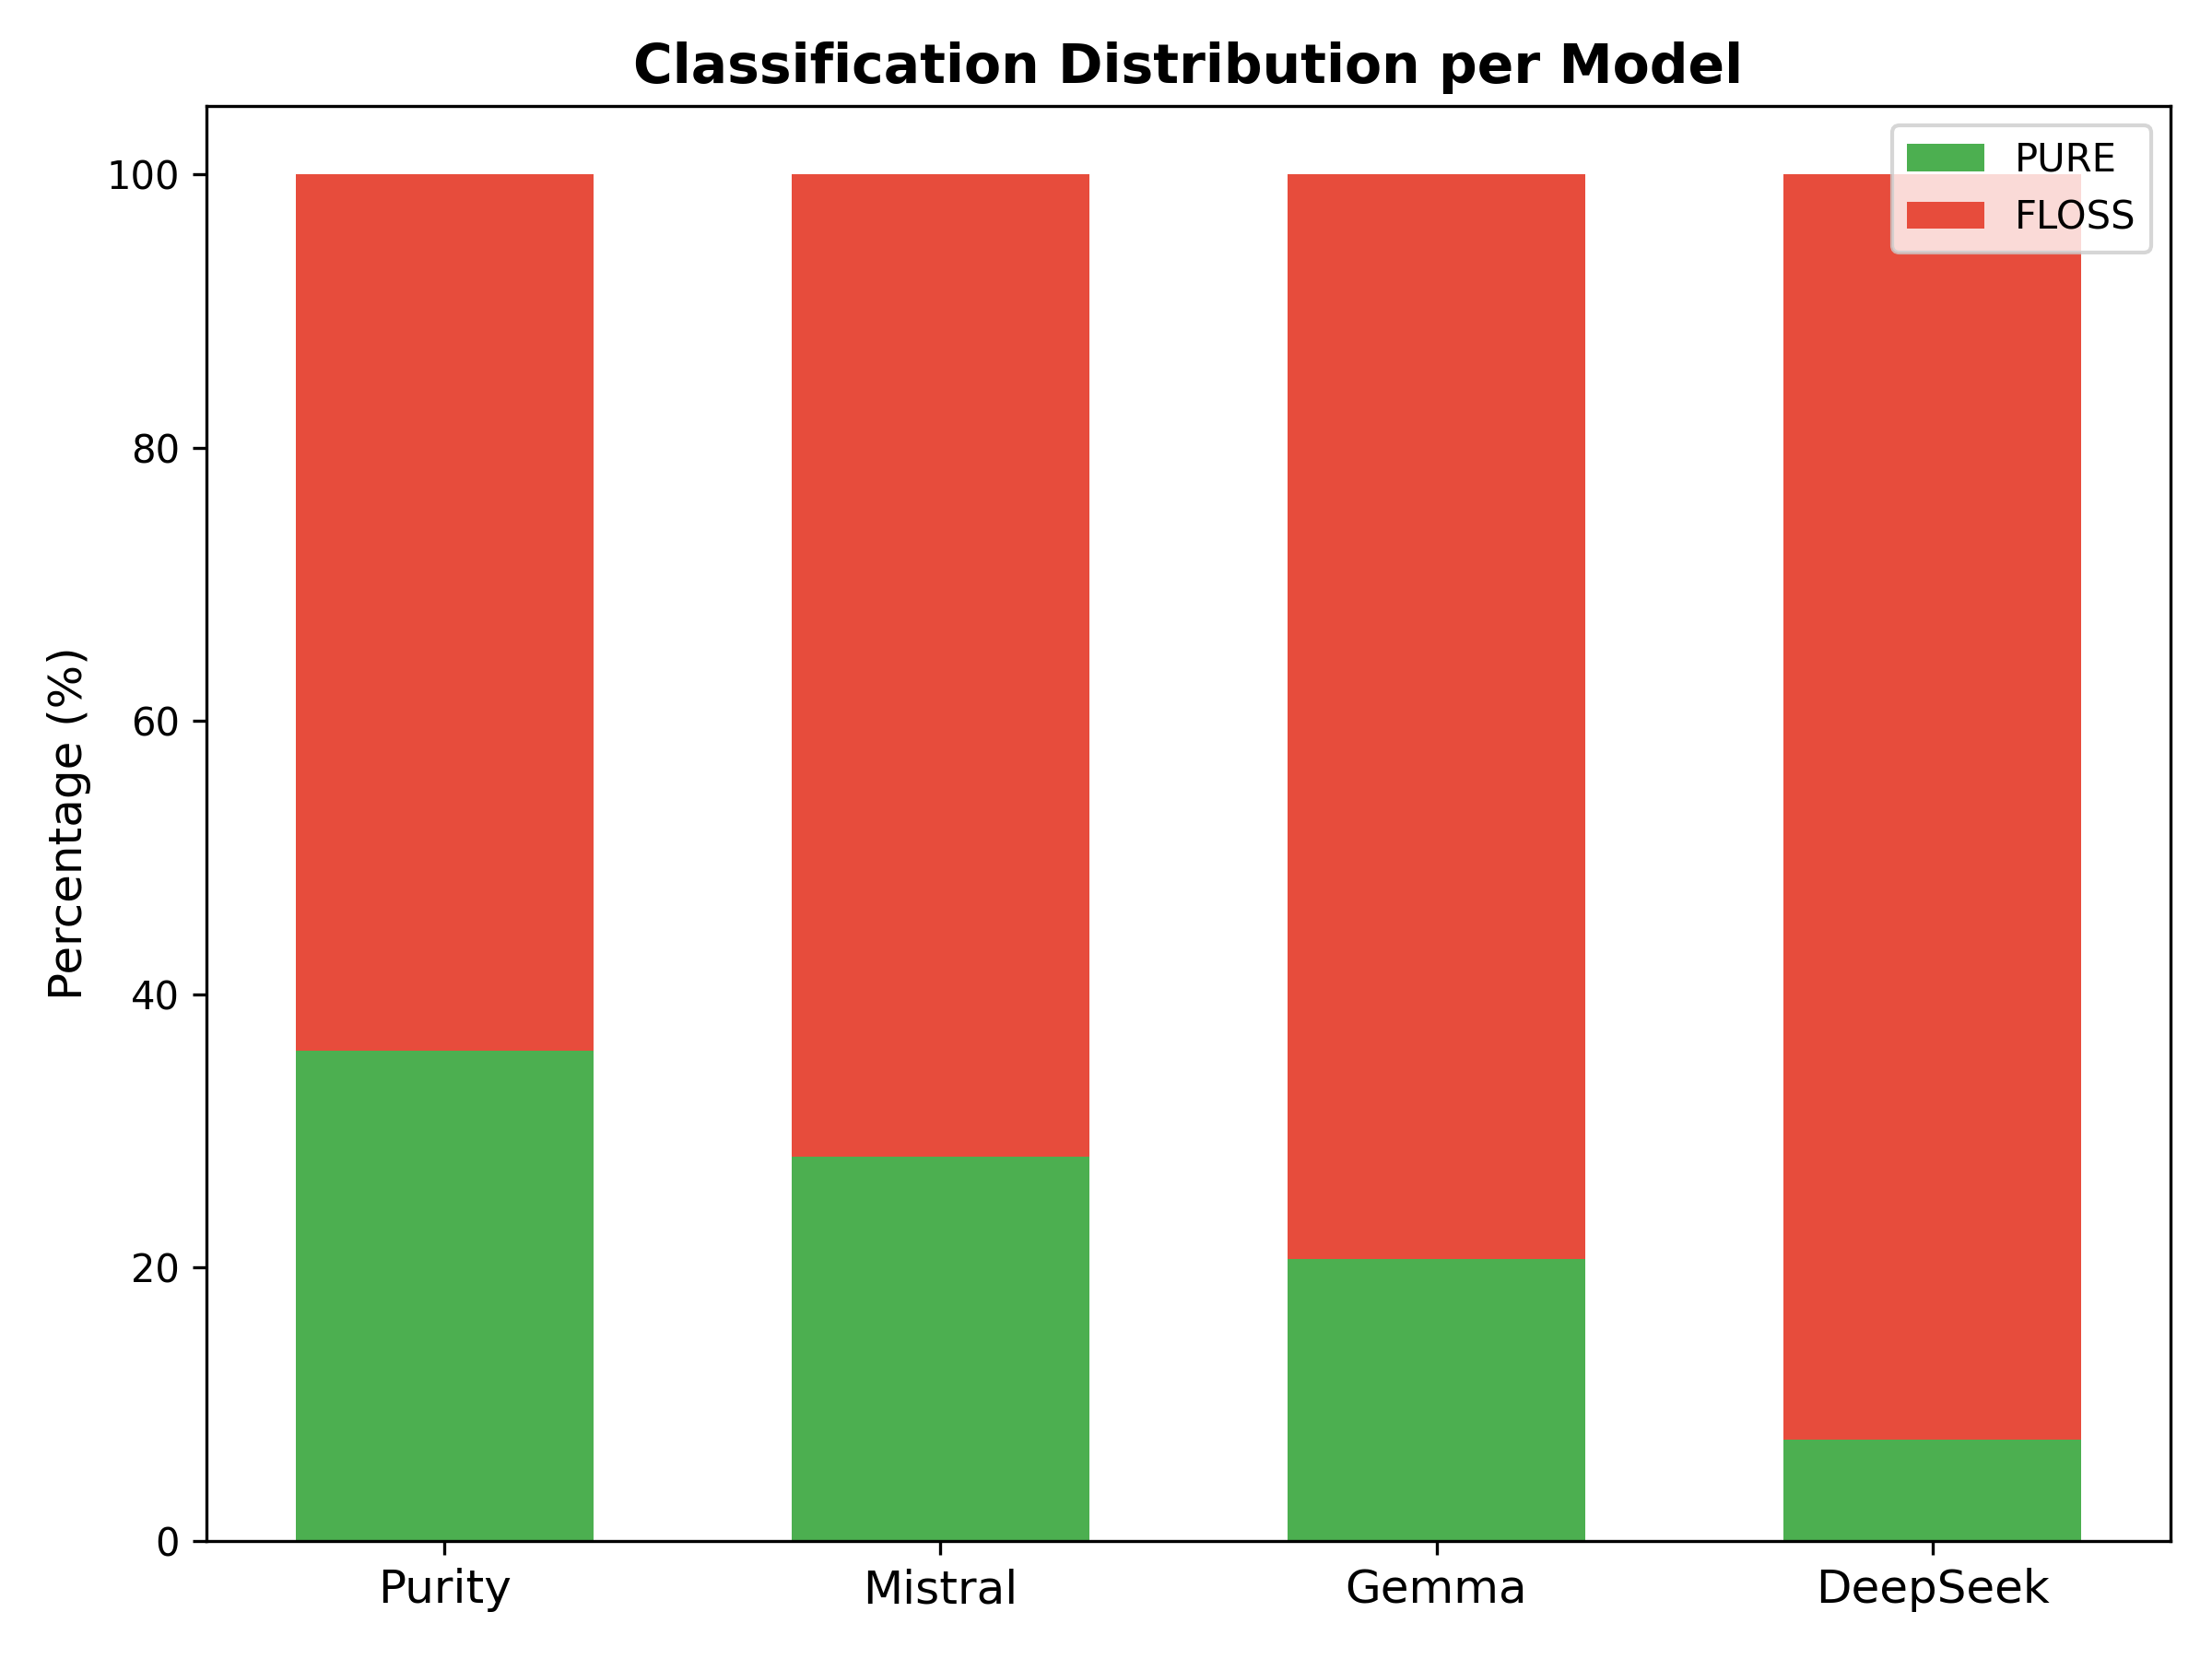
\includegraphics[width=0.6\textwidth]{fig/classification_distribution_models.png}
\caption{Distribution of PURE vs FLOSS classifications across Purity and the three LLMs. The LLMs tend to classify more commits as FLOSS compared to Purity.}
\label{fig:classification-distribution}
\end{figure}

Purity classified 35.85\% of commits as PURE and 64.15\% as FLOSS, reflecting its rule-based approach that identifies specific refactoring patterns. In contrast, the LLMs showed a progressive shift toward FLOSS classifications:
\begin{itemize}
    \item Mistral: 28.08\% PURE, 71.92\% FLOSS
    \item Gemma-2:2b: 20.56\% PURE, 79.44\% FLOSS
    \item DeepSeek-R1:8b: 7.37\% PURE, 92.63\% FLOSS
\end{itemize}

This pattern suggests that LLMs may be more cautious in identifying "pure" refactorings, potentially due to their training on diverse code patterns that make them sensitive to subtle behavioral changes. The extreme conservatism of DeepSeek-R1 (only 7.37\% PURE) indicates that larger models may prioritize safety over specificity in classification tasks.

\subsection{Agreement and Intersection Analysis}

To understand the relationships between different classification approaches, we analyzed pairwise and multi-way agreements. The Venn diagram in Figure~\ref{fig:venn} provides a visual representation of how classifications overlap across all four approaches.

\begin{figure}[H]
\centering
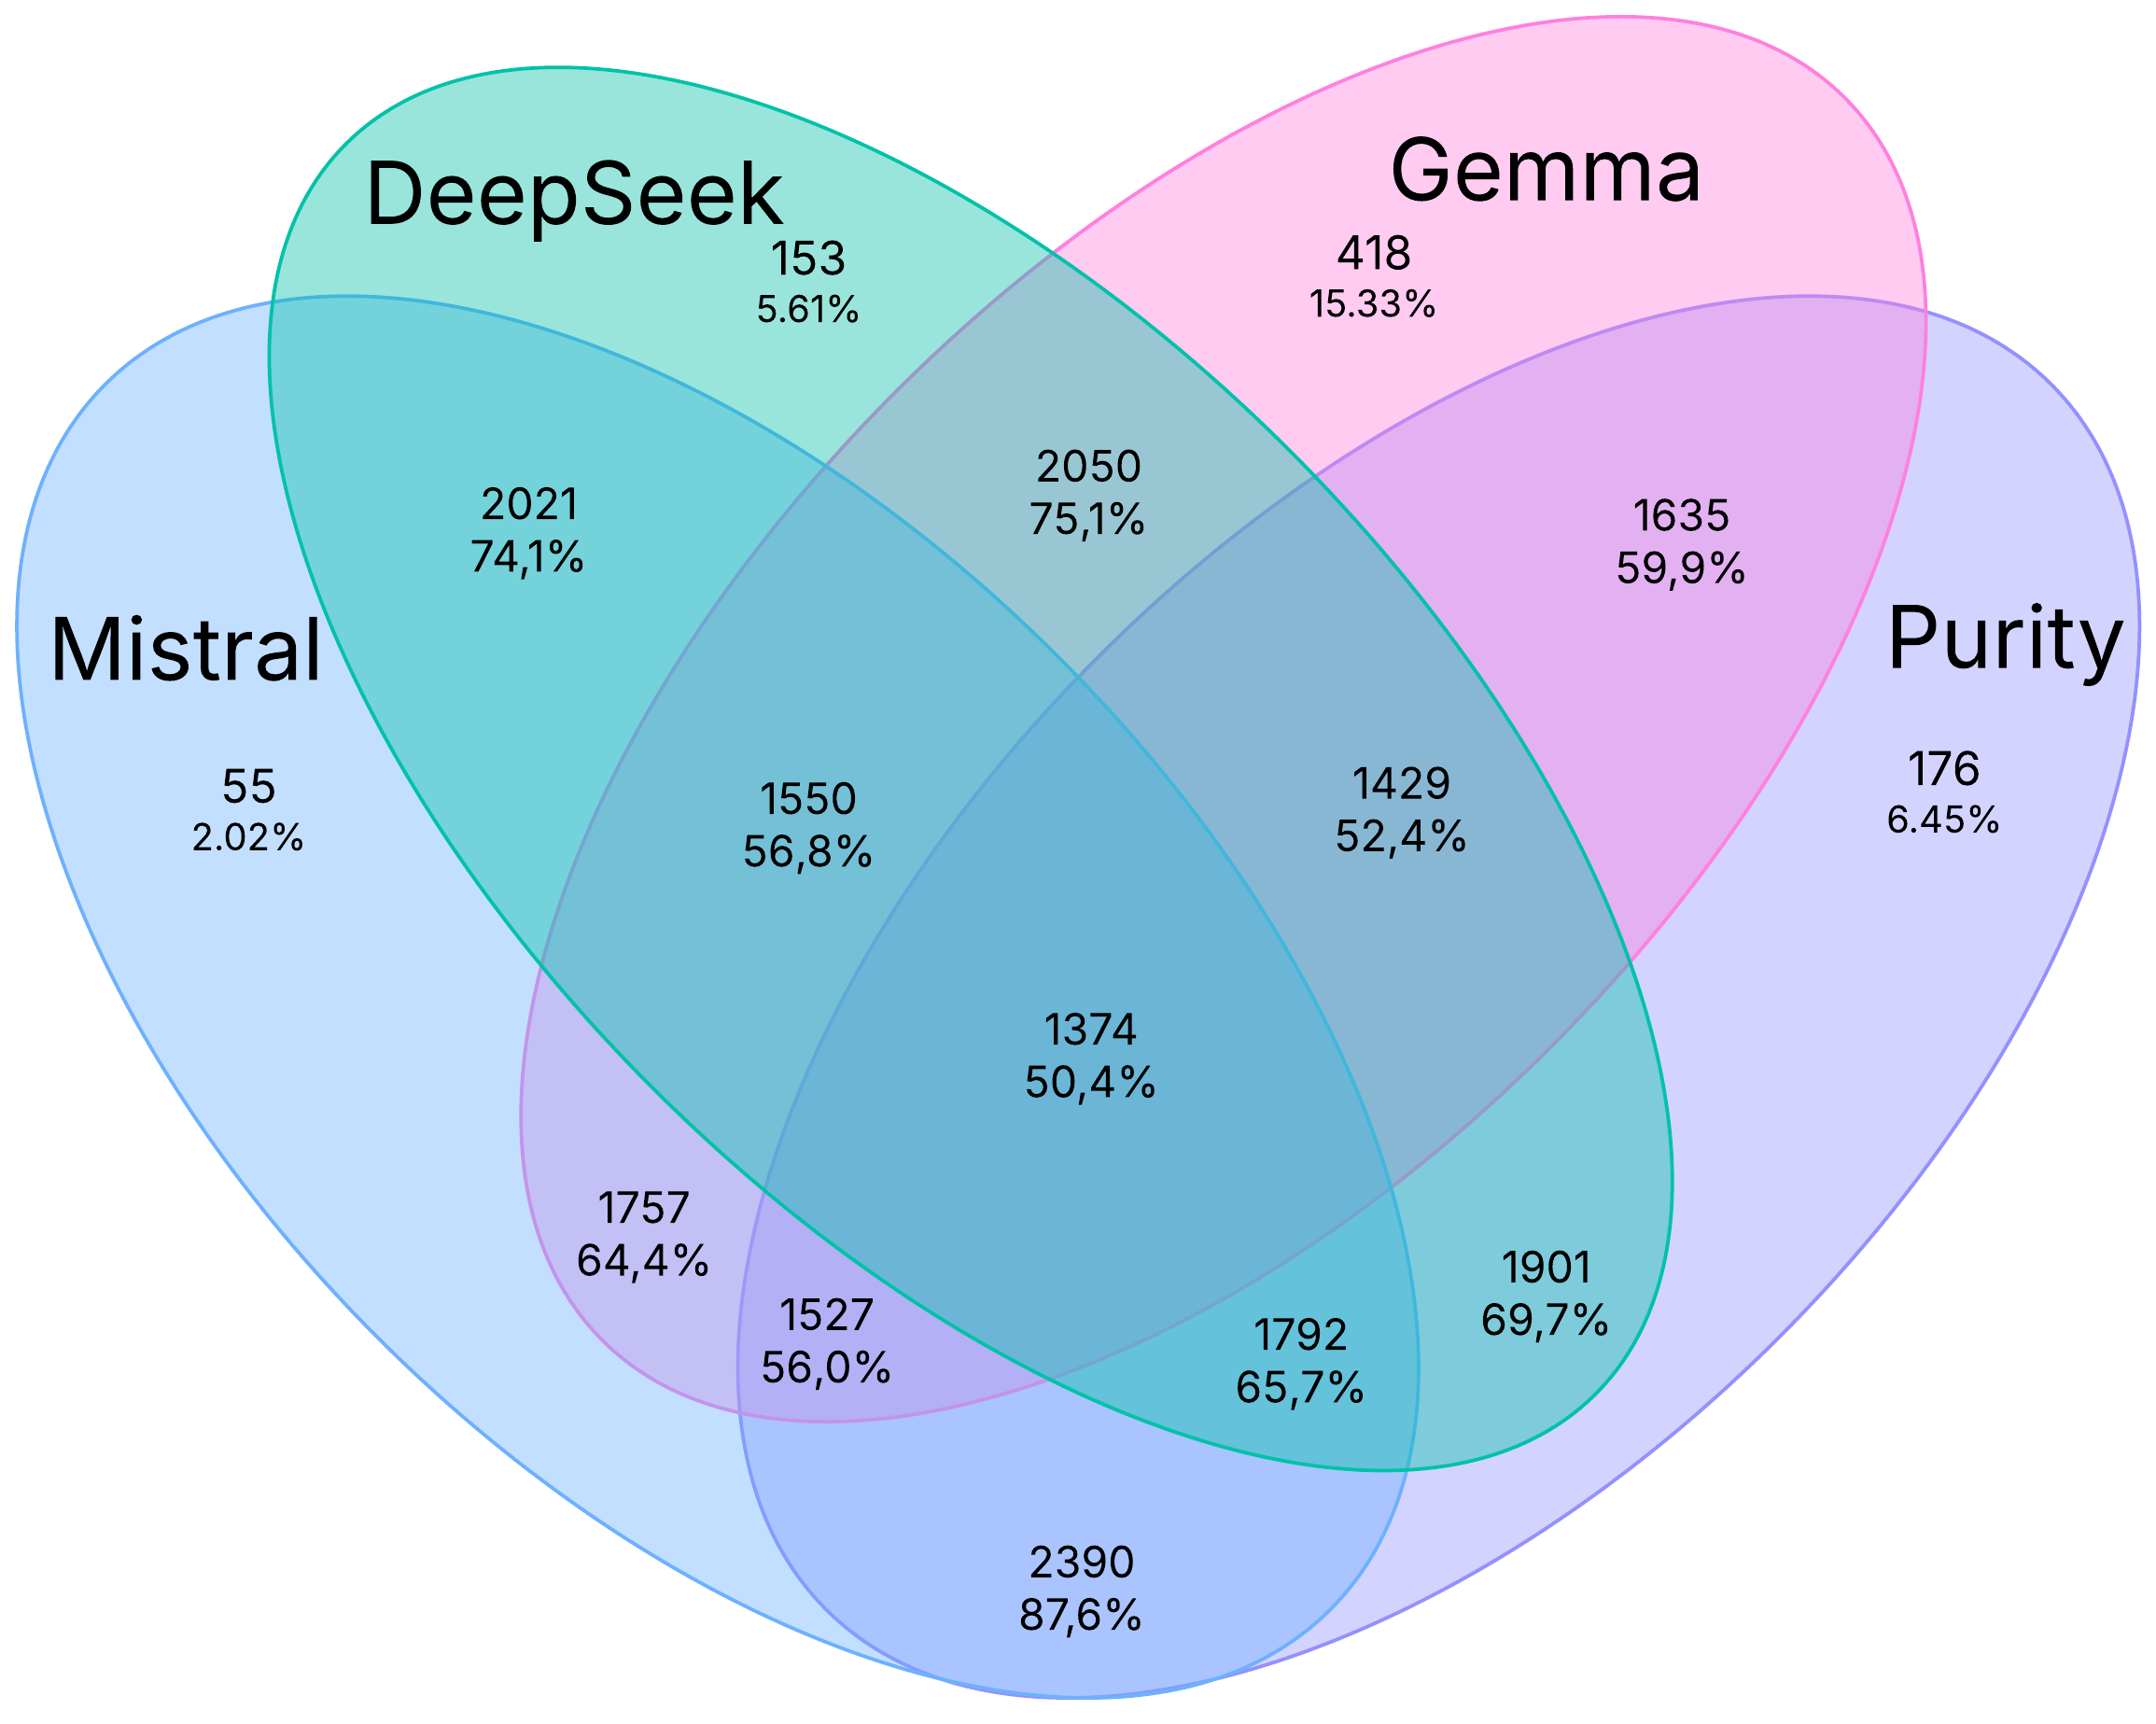
\includegraphics[width=0.7\textwidth]{fig/4-venn-complete.png}
\caption{Venn diagram showing intersections between Purity and LLM-based classifications. The diagram reveals both consensus areas and unique classifications by each approach.}
\label{fig:venn}
\end{figure}

The Venn diagram reveals several key insights:
\begin{itemize}
    \item A central region of consensus (50.37\% of commits) where all four classifiers agree
    \item Significant overlap between Purity and Mistral (87.61\% agreement)
    \item DeepSeek-R1 showing the most unique classifications, with substantial divergence from other approaches
    \item Gemma-2:2b positioned as a bridge between conservative (DeepSeek) and balanced (Mistral) approaches
\end{itemize}

Complementing the Venn diagram, the agreement heatmap (Figure~\ref{fig:agreement-heatmap}) quantifies pairwise similarities across all combinations.

\begin{figure}[H]
\centering
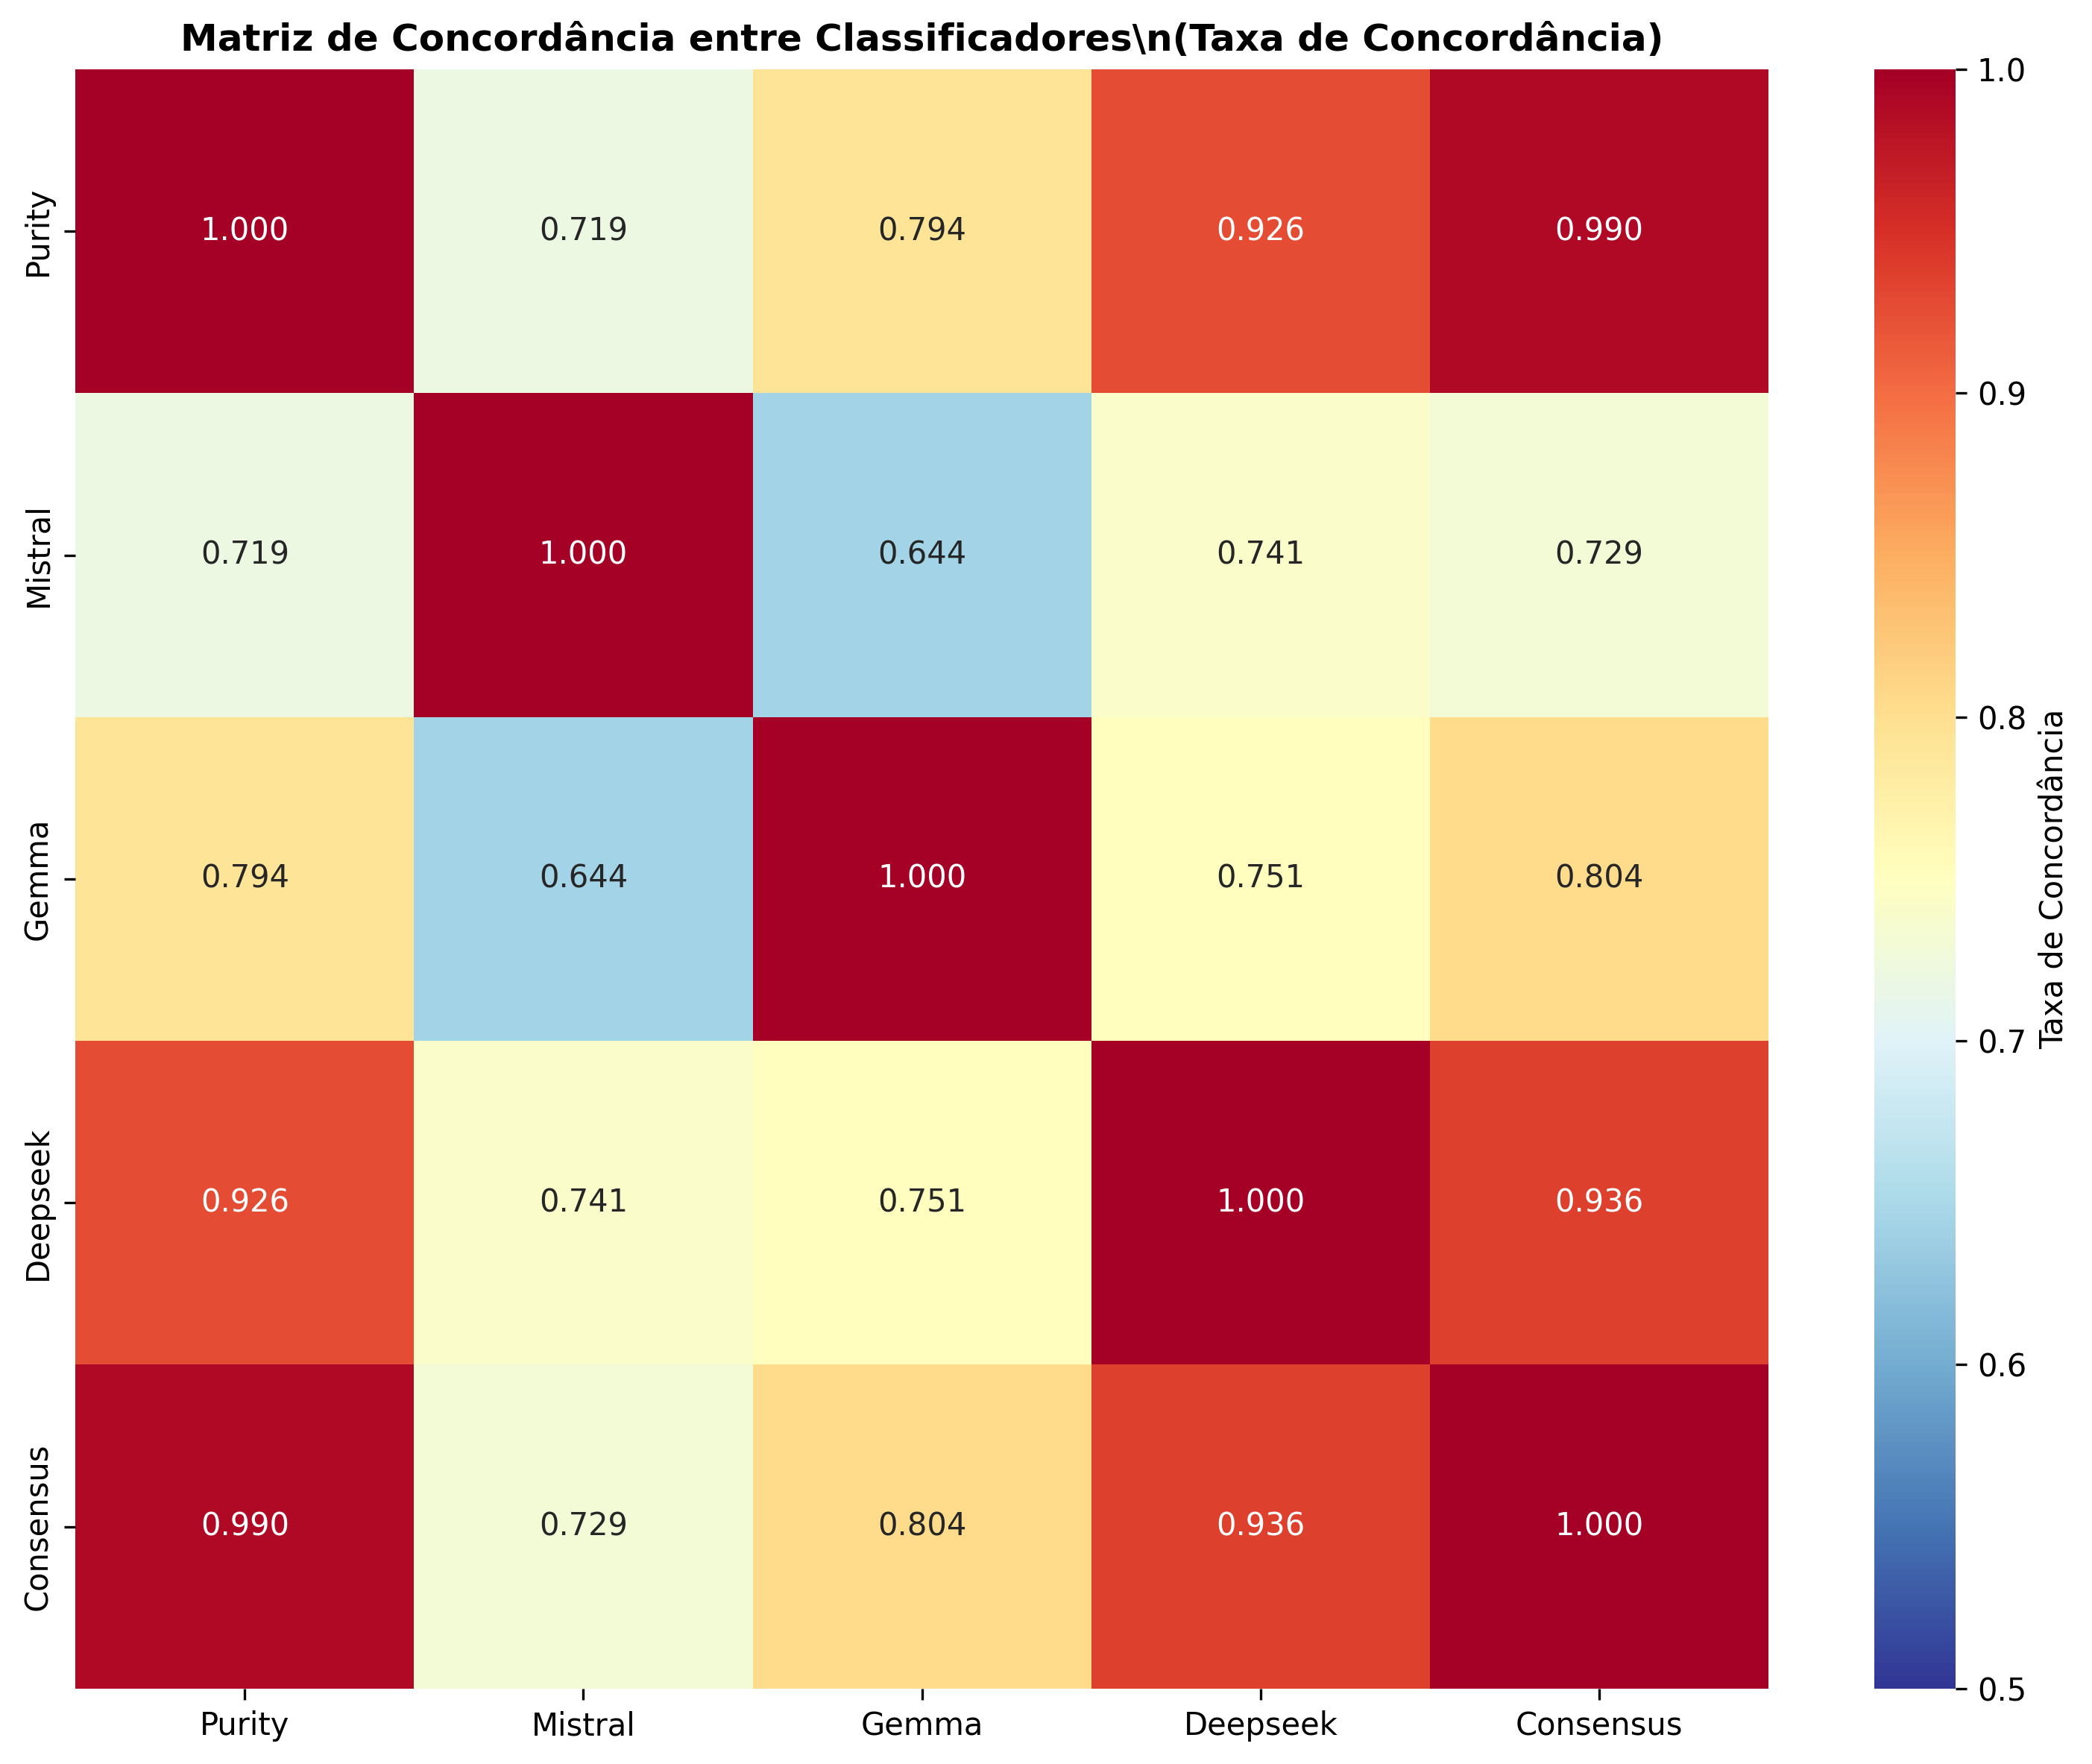
\includegraphics[width=0.6\textwidth]{fig/agreement_heatmap_fixed.png}
\caption{Agreement heatmap showing pairwise concordance rates between classifiers. Darker colors indicate higher agreement percentages.}
\label{fig:agreement-heatmap}
\end{figure}

The heatmap confirms the strong alignment between Purity and Mistral (87.61\% agreement), while highlighting DeepSeek-R1's divergence from traditional approaches. This analysis suggests that Mistral's architecture may be particularly well-suited for refactoring classification tasks, potentially due to its balance of model size and training objectives.

\subsection{Consensus Analysis}

Consensus analysis provides a robust measure of classification reliability by examining agreements across multiple independent approaches. Figure~\ref{fig:consensus-distribution} shows the distribution of consensus outcomes when considering all four classifiers.

\begin{figure}[H]
\centering
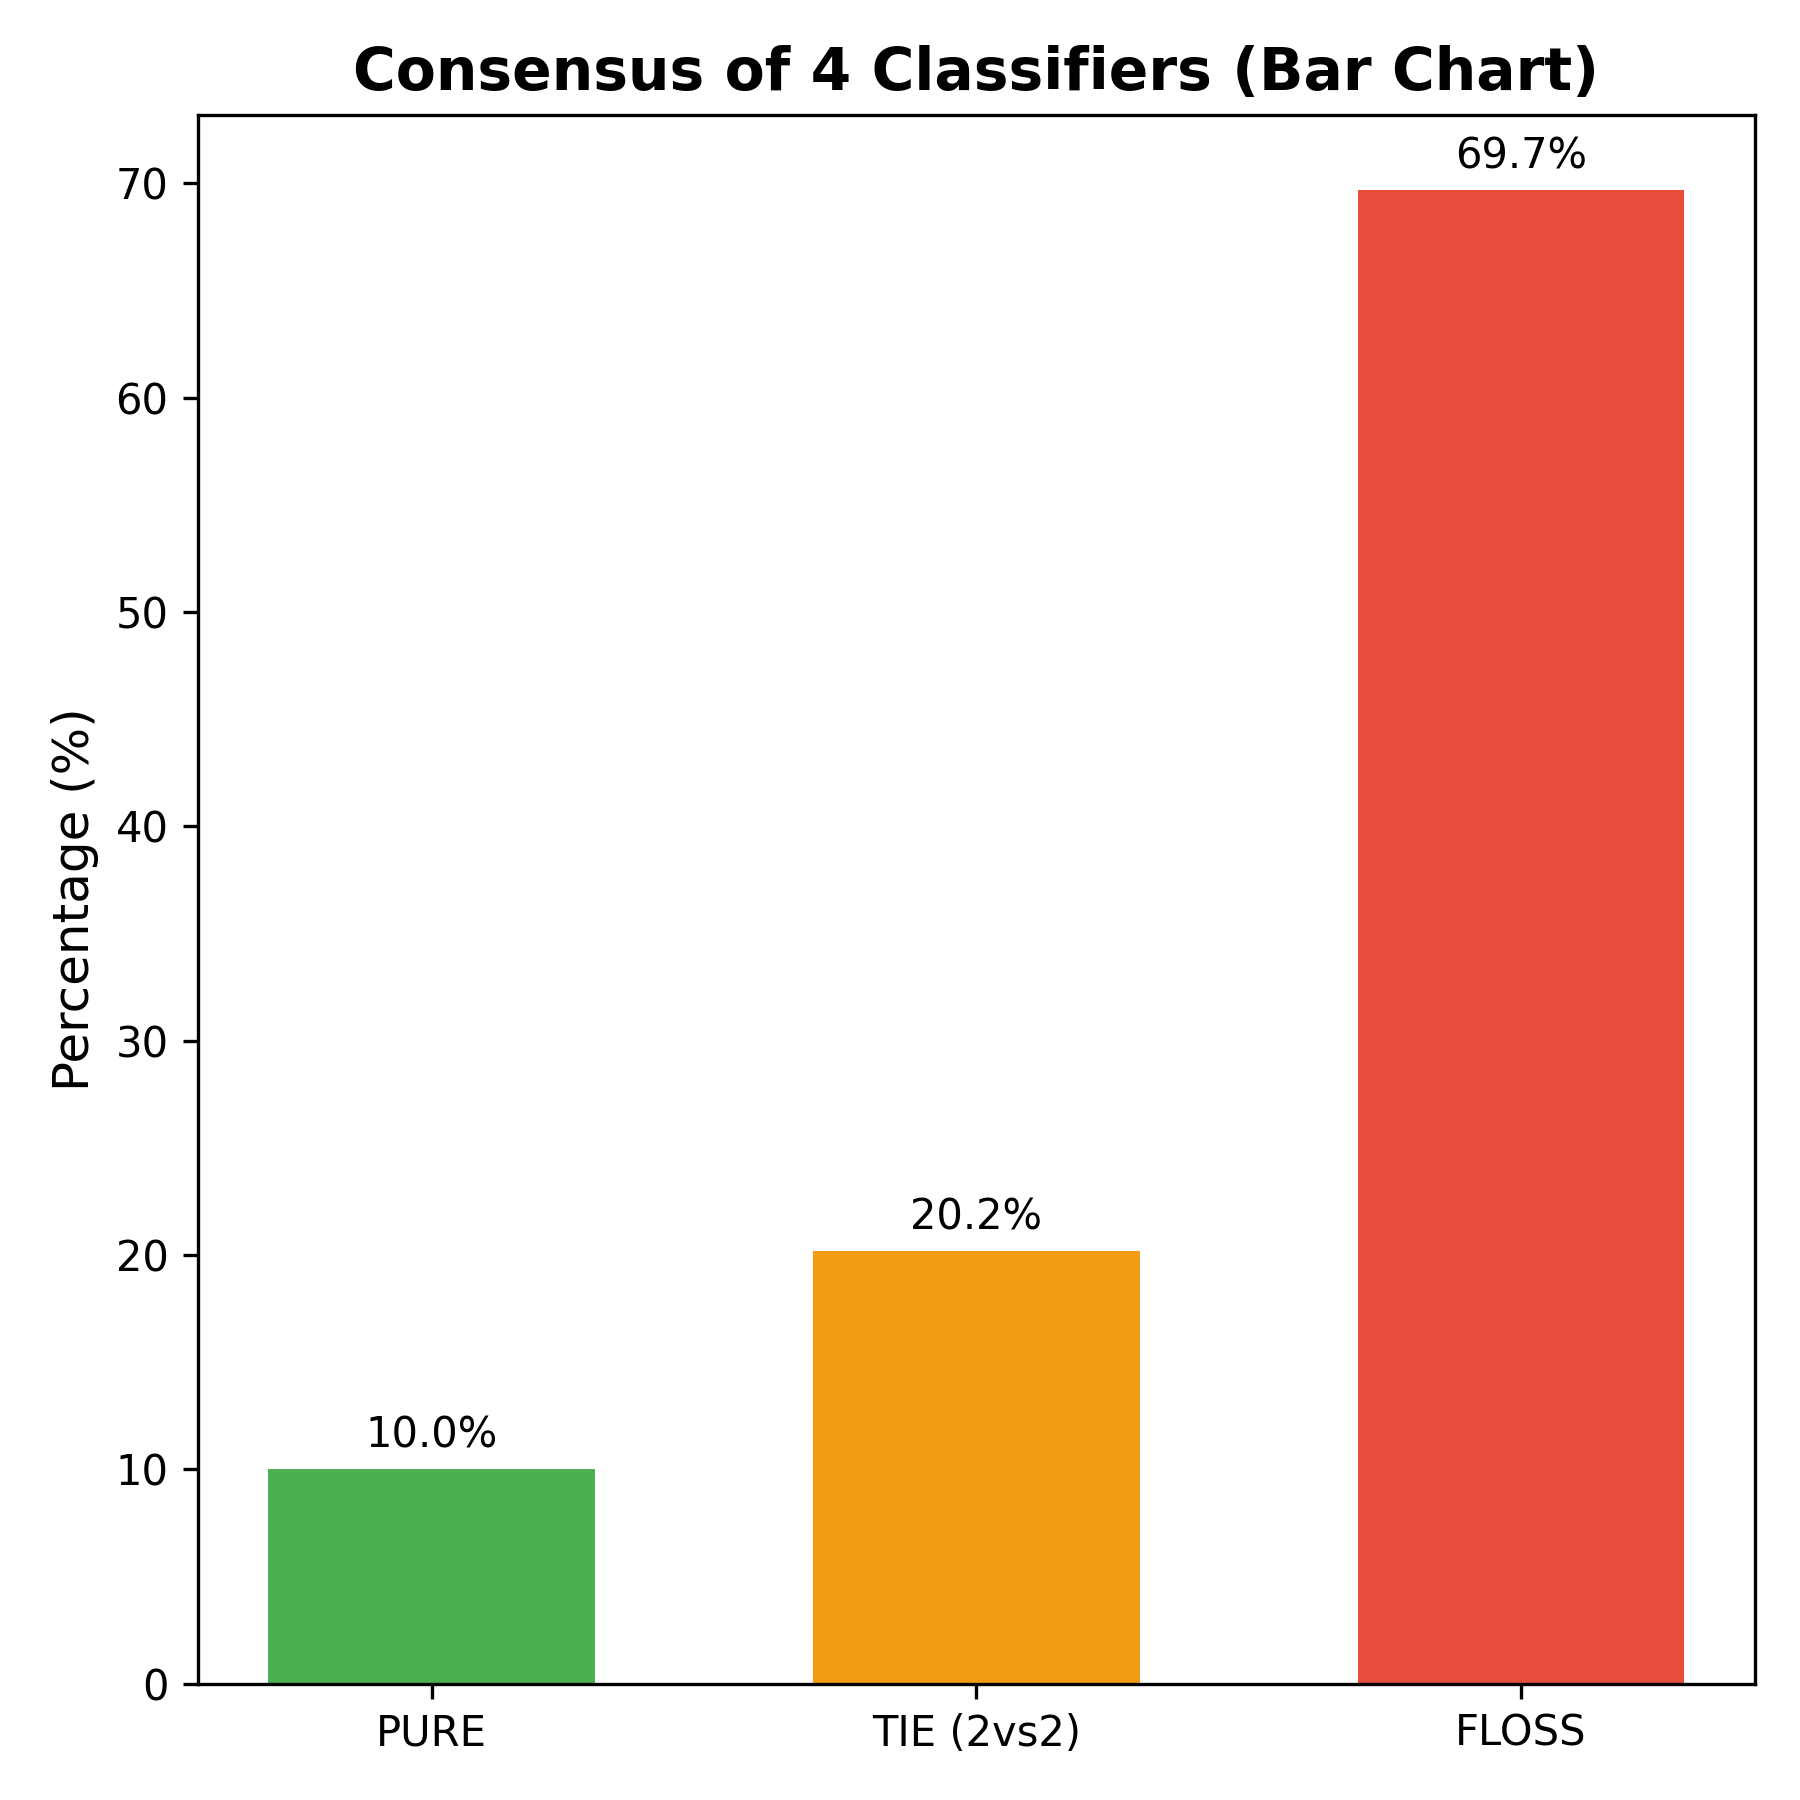
\includegraphics[width=0.6\textwidth]{fig/consensus_bar.png}
\caption{Distribution of consensus classifications across PURE, FLOSS, and TIE categories. The chart shows the proportion of commits where multiple classifiers agree.}
\label{fig:consensus-distribution}
\end{figure}

Key findings from the consensus analysis are summarized in Table~\ref{tab:consensus-findings}.

\begin{table}[ht]
\centering
\caption{Key findings from consensus analysis across all classifiers.}
\label{tab:consensus-findings}
\begin{tabular}{@{}p{0.25\textwidth}p{0.15\textwidth}p{0.4\textwidth}@{}}
\toprule
\textbf{Consensus Type} & \textbf{Percentage} & \textbf{Description} \\
\midrule
Absolute consensus & 50.37\% & All four classifiers agree \\
At least three agree & 65.69\% & Agreement among Purity + Mistral + DeepSeek \\
FLOSS consensus & 49.41\% & Dominant consensus outcome \\
PURE consensus & 0.95\% & Rare consensus on pure refactorings \\
\bottomrule
\end{tabular}
\end{table}

The predominance of FLOSS consensus suggests that when classifiers disagree, they tend to err on the side of caution, classifying ambiguous refactorings as potentially behavior-altering. This conservative bias may be beneficial for quality assurance but could limit the identification of truly pure refactorings.

\subsection{Failure Rate Analysis}

While LLMs offer sophisticated classification capabilities, they also introduce practical challenges related to output reliability. Figure~\ref{fig:failed-percentages} illustrates the failure rates across different models, where failures represent instances of invalid or incomplete JSON output.

\begin{figure}[H]
\centering
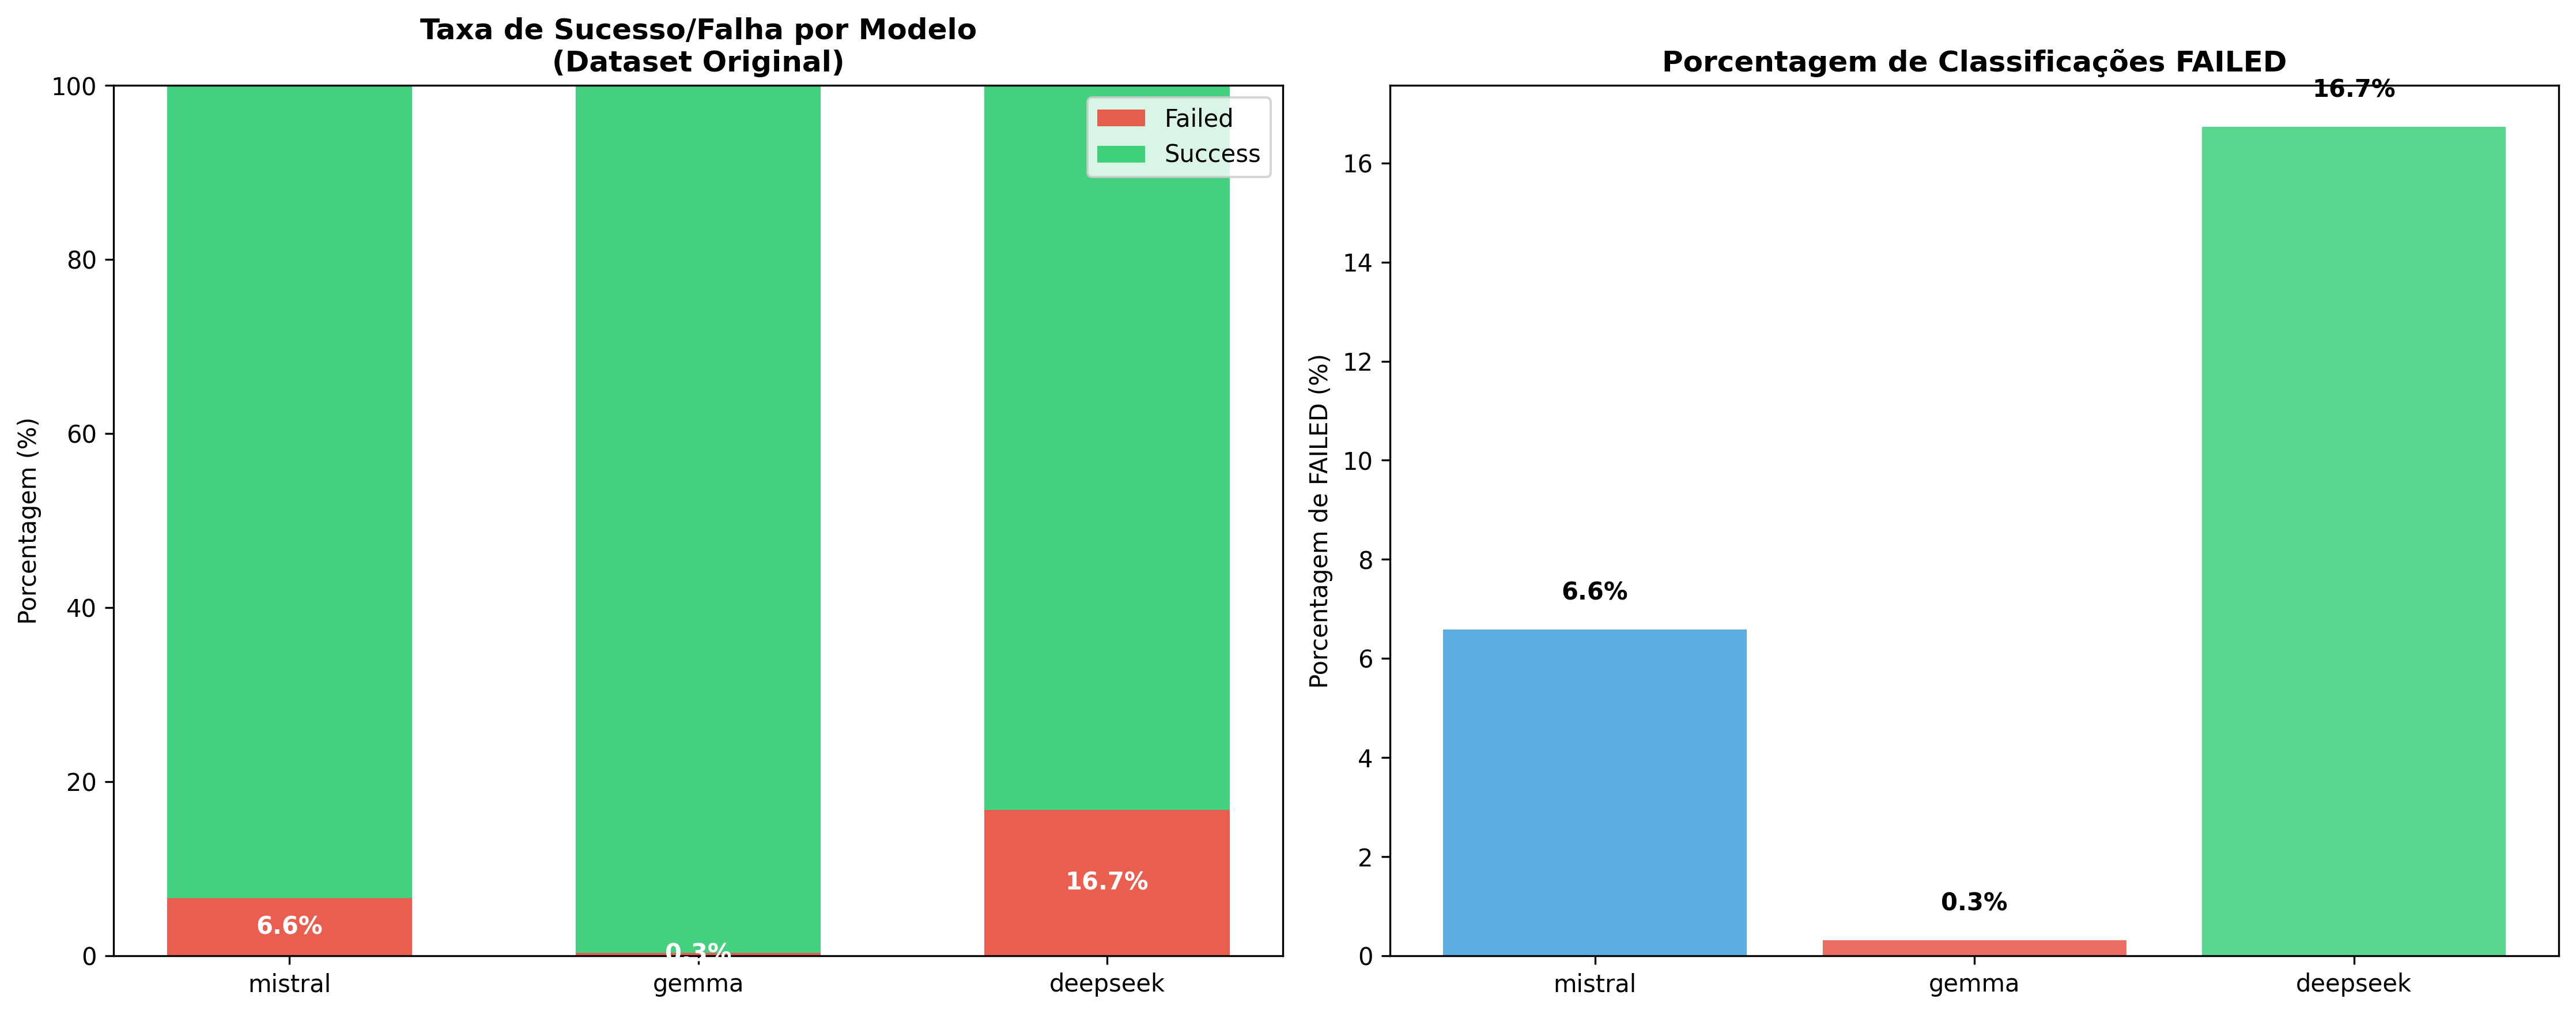
\includegraphics[width=0.6\textwidth]{fig/failed_percentages_ultimate.png}
\caption{Failure rates across models showing the proportion of commits that resulted in invalid outputs. Lower failure rates indicate more robust model behavior.}
\label{fig:failed-percentages}
\end{figure}

The failure analysis reveals important trade-offs:
\begin{itemize}
    \item Gemma-2:2b demonstrates the lowest failure rate, suggesting better output stability
    \item DeepSeek-R1 shows higher failure rates, potentially due to its larger size and complexity
    \item Mistral provides a good balance between low failure rates and classification accuracy
    \item Output format reliability is crucial for production deployment of LLM-based classifiers
\end{itemize}

\subsection{Manual Analysis of Disagreements}

To gain deeper insights into classification differences, we conducted a manual analysis of specific disagreement patterns. This qualitative examination focused on three key scenarios:

\subsubsection{Discordance: Purity PURE vs. LLM FLOSS Consensus}

In cases where Purity classified a commit as PURE but all three LLMs agreed on FLOSS, we identified common patterns:
\begin{itemize}
    \item Subtle API changes that LLMs interpreted as behavioral modifications
    \item Complex refactoring sequences that exceeded LLM context understanding
    \item Documentation updates accompanying code changes that influenced LLM judgment
\end{itemize}

\subsubsection{Tie Scenarios: 2-2 Agreement Splits}

When classifiers split evenly (e.g., Purity + Mistral vs. Gemma + DeepSeek), the disagreements often stemmed from:
\begin{itemize}
    \item Ambiguous commit messages that could be interpreted differently
    \item Mixed refactoring and feature addition patterns
    \item Language-specific idioms that different models processed variably
\end{itemize}

\subsubsection{Purity NONE Classifications}

For commits that Purity classified as NONE (non-refactoring), the LLMs showed varied responses:
\begin{itemize}
    \item Mistral most frequently agreed with NONE classifications
    \item Gemma and DeepSeek tended to classify such commits as FLOSS
    \item This suggests different sensitivity thresholds for identifying refactoring intent
\end{itemize}

\subsection{Discussion}

Our comprehensive evaluation provides clear answers to the research questions posed at the outset of this study. We discuss these findings in detail below, followed by broader implications and future research directions.

\subsubsection{Response to RQ1: LLM Accuracy Compared to Purity}

RQ1 asked: "To what extent can Large Language Models classify refactoring commits (PURE vs. FLOSS) with accuracy comparable to the established Purity tool?"

Our results demonstrate that LLMs can achieve classification performance comparable to Purity, with notable variations across models. The strongest alignment was observed between Purity and Mistral, which agreed on 87.61\% of classifications. This high concordance rate suggests that Mistral's architecture and training data make it particularly effective for refactoring classification tasks.

However, the comparison reveals systematic differences in classification behavior:
\begin{itemize}
    \item \textbf{Purity's Approach:} Rule-based system that identifies specific refactoring patterns, resulting in 35.85\% PURE and 64.15\% FLOSS classifications
    \item \textbf{LLM Tendencies:} More conservative approach, with Mistral (71.92\% FLOSS), Gemma (79.44\% FLOSS), and DeepSeek (92.63\% FLOSS) showing progressive increases in FLOSS classifications
\end{itemize}

The consensus analysis further supports LLM competitiveness, with 50.37\% absolute agreement across all four classifiers and 65.69\% agreement among at least three approaches. These findings indicate that LLMs can match Purity's accuracy while offering complementary strengths in handling complex or ambiguous refactoring scenarios.

\subsubsection{Response to RQ2: Variations Across Different LLMs}

RQ2 asked: "How do different LLMs (Gemma-2:2b, Mistral, DeepSeek-R1:8b) vary in their classification performance, and what factors influence these differences?"

Our analysis reveals significant variations across the three LLMs, influenced by model size, architecture, and training objectives:

\begin{itemize}
    \item \textbf{Mistral (Balanced Performer):} Demonstrated the strongest alignment with Purity (87.61\% agreement) and most balanced classification distribution (28.08\% PURE). Its moderate size and optimized architecture appear to provide the best trade-off between accuracy and efficiency.
    
    \item \textbf{Gemma-2:2b (Conservative Classifier):} Showed more conservative behavior (79.44\% FLOSS) with reasonable agreement rates (59.93\% with Purity). The smaller model size contributes to lower failure rates but also more cautious classification.
    
    \item \textbf{DeepSeek-R1:8b (Highly Conservative):} Exhibited extreme conservatism (92.63\% FLOSS) with the lowest PURE classification rate (7.37\%). While showing substantial divergence from traditional approaches, it also demonstrated higher failure rates, suggesting that larger models may prioritize safety over specificity.
\end{itemize}

Key factors influencing these differences include:
\begin{itemize}
    \item \textbf{Model Size:} Larger models (DeepSeek) tend toward more conservative classifications
    \item \textbf{Training Objectives:} Models optimized for different tasks show varying sensitivity to refactoring patterns
    \item \textbf{Architecture:} Different transformer architectures affect how models process code and commit context
    \item \textbf{Output Stability:} Smaller models generally show more reliable JSON output generation
\end{itemize}

\subsubsection{Broader Implications and Strengths of LLM-Based Classification}

Beyond addressing the specific research questions, our findings highlight several advantages of LLM-based approaches:

\begin{itemize}
    \item \textbf{Flexibility:} LLMs can handle complex, nuanced refactoring patterns that rigid rules might miss
    \item \textbf{Context Awareness:} Models consider commit messages and code context holistically
    \item \textbf{Adaptability:} LLMs can potentially learn from new refactoring patterns without manual rule updates
    \item \textbf{Scalability:} Once configured, LLMs can process large volumes of commits efficiently
\end{itemize}

\subsubsection{Limitations and Challenges}

Despite promising results, several challenges remain:

\begin{itemize}
    \item \textbf{Conservative Bias:} LLMs tend to classify ambiguous cases as FLOSS, potentially missing pure refactorings
    \item \textbf{Output Reliability:} JSON parsing failures and format inconsistencies require robust error handling
    \item \textbf{Computational Cost:} Larger models like DeepSeek-R1 demand significant resources
    \item \textbf{Interpretability:} Unlike rule-based systems, LLM decisions are not easily explainable
\end{itemize}

\subsubsection{Practical Implications}

The strong agreement between Purity and Mistral (87.61\%) suggests that carefully selected LLMs can serve as reliable classification tools in software engineering workflows. The consensus analysis indicates that combining multiple approaches could further improve reliability, with 65.69\% agreement among three classifiers.

For practical deployment, we recommend:
\begin{itemize}
    \item Using Mistral for balanced performance between accuracy and efficiency
    \item Implementing robust error handling and retry mechanisms
    \item Combining LLM classifications with traditional tools for critical decisions
    \item Regular validation against human expert judgments
\end{itemize}

\subsubsection{Future Research Directions}

Our findings open several avenues for future work:
\begin{itemize}
    \item Fine-tuning LLMs specifically for refactoring classification tasks
    \item Developing hybrid approaches combining rule-based and LLM methods
    \item Exploring the impact of different prompt engineering strategies
    \item Extending the analysis to other programming languages and refactoring types
\end{itemize}

\subsection{Conclusion}

This study demonstrates that LLMs can achieve classification performance comparable to established tools like Purity, with Mistral showing particularly strong alignment (87.61\% agreement). While challenges remain in output reliability and conservative bias, the flexibility and context-awareness of LLMs make them promising tools for automated refactoring analysis. The consensus analysis suggests that combining multiple approaches could provide even more robust classification, paving the way for more sophisticated software engineering automation tools.

\begin{figure}[H]
\centering
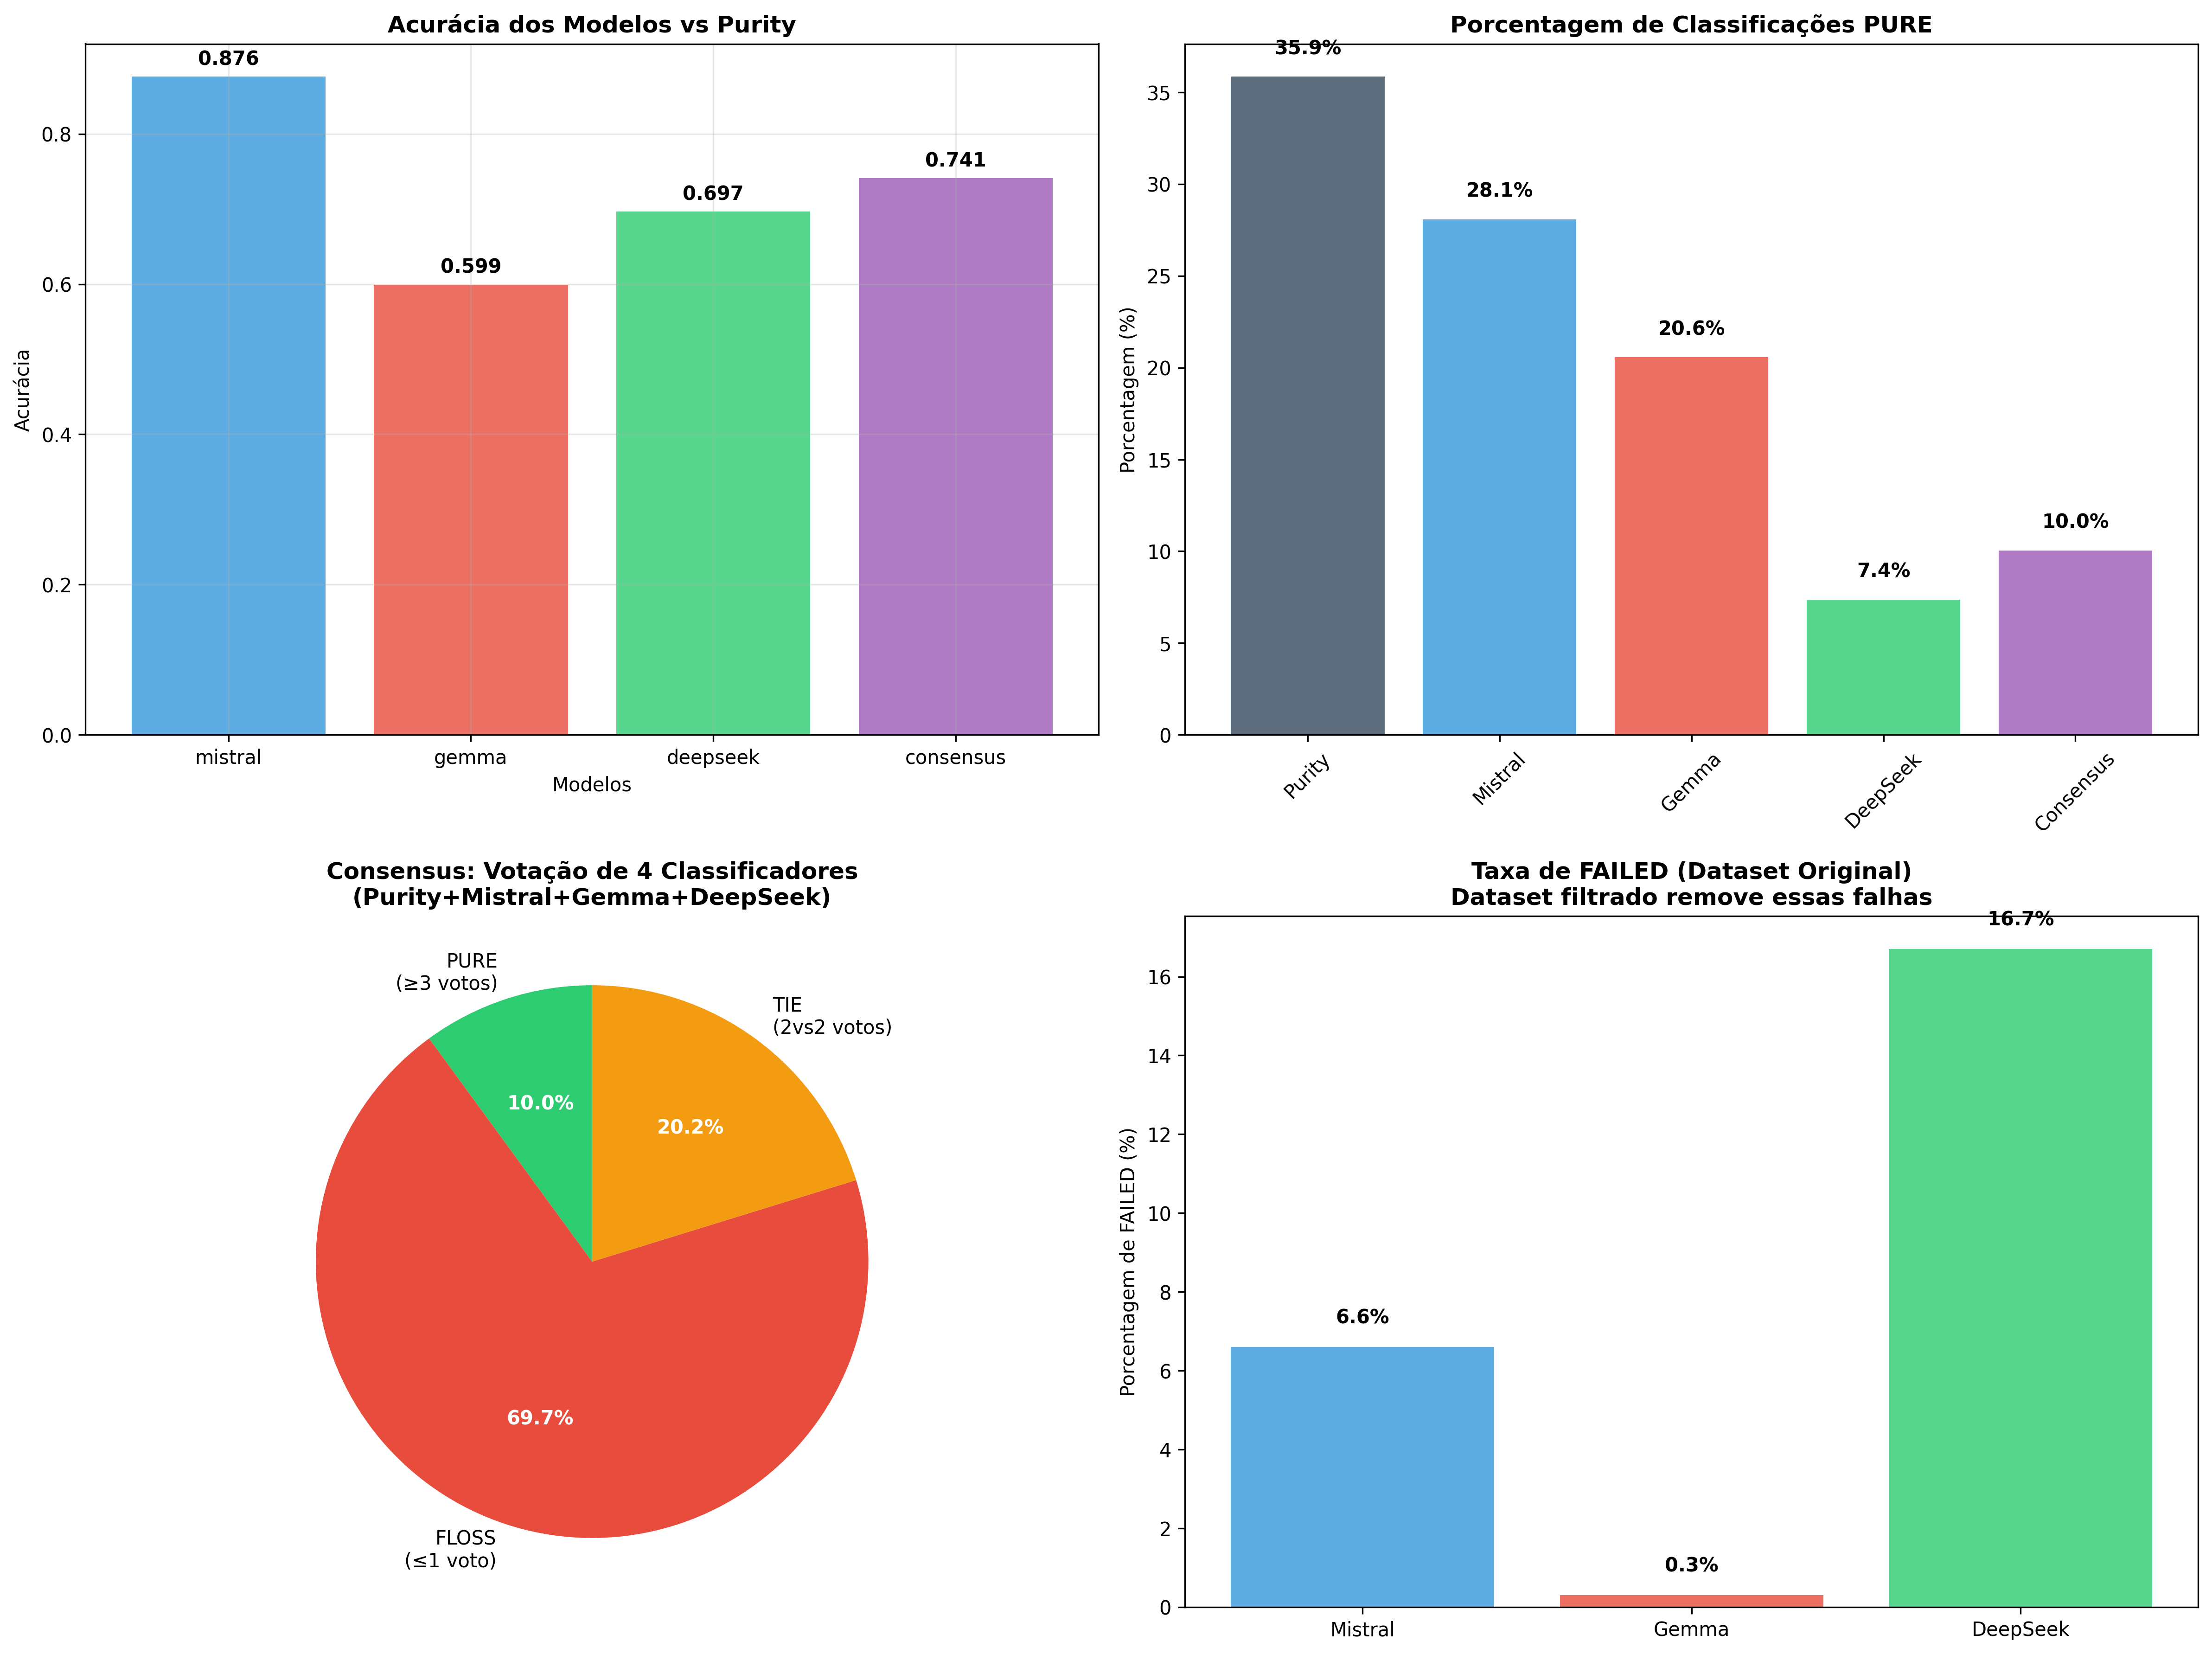
\includegraphics[width=0.8\textwidth]{fig/analysis_summary_ultimate.png}
\caption{Summary of key findings: classification distributions, agreement patterns, and performance trade-offs across all models.}
\label{fig:analysis-summary}
\end{figure}